\chapter{Quotient Space and Simplicial Complex}

In the end of Chapter 2, we introduced product space and disjoint union. In this Chapter, we give another way to construct new topological spaces from some old ones. This new way of construction is by gluing some special pieces from old topological spaces together.

The rough idea is as follows: Let \(X = \left\lbrack  {0,1}\right\rbrack   \times  \left\lbrack  {0,1}\right\rbrack\) (just like a piece of paper on a plane), we want to glue the leftmost edge with the rightmost edge to form a cylinder \({Y}_{1}\), as shown below:

\begin{center}
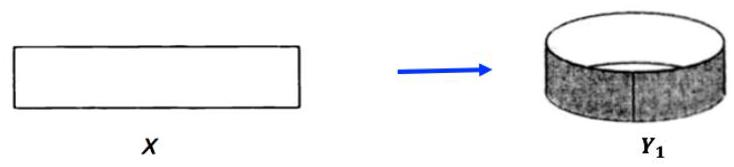
\includegraphics[width=0.5\textwidth]{images/Ch4_cylinder.jpg}
\end{center}
\hspace*{3em} 

If we give a half-twist to the strip before glue the ends together, we will get the Moebius strip \({Y}_{2}\) shown below:

\begin{center}
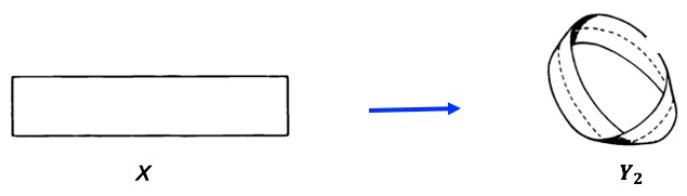
\includegraphics[width=0.5\textwidth]{images/Ch4_mobius1.jpg}
\end{center}
\hspace*{3em} 

Interestingly, the first topology \({Y}_{1}\) has two sides, while the second has only one side.

\section{Equivalence Relations and Equivalence Classes}

\begin{definition}[Equivalence Relation] \label{def:equiv_relation} The equivalence relation on a set \(X\) is a relation \~ such that

1. (Reflexive): \(x \sim  x,\forall x \in  X\)

2. (Symmetric): \(x \sim  y\) implies \(y \sim  x\)

3. (Transitive): \(x \sim  y\) and \(y \sim  z\) implies \(x \sim  z\).
\end{definition}

\begin{example} \label{eg:equiv_relation} 1. Let \(X = V\) be a vector space, and \(W \leq  V\) be a vector subspace. Define \({\mathbf{v}}_{1} \sim  {\mathbf{v}}_{2}\) if \({\mathbf{v}}_{1} - {\mathbf{v}}_{2} \in  W\).
(The well-definedness is left as exercise).

2. (Mobius Strip): Let \(X = \left\lbrack  {0,1}\right\rbrack   \times  \left\lbrack  {0,1}\right\rbrack\). We define \(\left( {{x}_{1},{y}_{1}}\right)  \sim  \left( {{x}_{2},{y}_{2}}\right)\) if

\begin{itemize}
\item \({x}_{1} = {x}_{2},{y}_{1} = {y}_{2}\) ; (e.g., \(\left( {{0.5},{0.6}}\right)  \sim  \left( {{0.5},{0.6}}\right)\) ) or
\end{itemize}

\begin{itemize}
\item \({x}_{1} = 0,{x}_{2} = 1\), and \({y}_{1} = 1 - {y}_{2}\) (e.g., \(\left( {0,1/4}\right)  \sim  \left( {1,3/4}\right)\) )
\end{itemize}

\begin{itemize}
\item \({x}_{1} = 1,{x}_{2} = 0\), and \({y}_{1} = 1 - {y}_{2}\) (e.g., \(\left( {1,3/4}\right)  \sim  \left( {0,1/4}\right)\) )
\end{itemize}
\end{example}

Another way to define an equivalence relation is to use partitions:
\begin{definition}[Partition] Let \(X\) be a nonempty set. A partition \(\mathcal{P} = \left\{  {{p}_{i} \mid  i \in  I}\right\}\) of \(X\) is a collection of subsets such that

1. \({P}_{i} \subseteq  X\) is non-empty

2. \({P}_{i} \cap  {P}_{j} = \varnothing\) if \(i \neq  j\)

3. \(\mathop{\bigcup }\limits_{{i \in  I}}{P}_{i} = X\).

Given a partition \(\mathcal{P} = \left\{  {{p}_{i} \mid  i \in  I}\right\}\), we can define an equivalence relation \(\sim\) on \(X\) by setting
\[
x \sim  y\;\text{ whenever }x,y \in  {p}_{i}\text{, for some }i \in  I
\]
\end{definition}
\begin{example}
Let \(X = \left\lbrack  {0,1}\right\rbrack   \times  \left\lbrack  {0,1}\right\rbrack\).
Then the partition 
\[
X = \{ \left( {x,y}\right) {\} }_{x \in  \left( {0,1}\right),y \in  \left\lbrack  {0,1}\right\rbrack  } \cup  \{ \left( {1,y}\right),\left( {0,1 - y}\right) {\} }_{y \in  \left\lbrack  {0,1}\right\rbrack  }
\]
gives the same equivalence relation as in part (2) in \autoref{eg:equiv_relation}.    
\end{example}

Conversely, for any equivalence relation \(\sim\) of $X$, we could form a corresponding partition of \(X\). This kind of partition is called the equivalence class:
\begin{definition}[Equivalence Class] Let \(X\) be a set with equivalence relation \(\sim\). The {\bf equivalence class} of an element \(x \in  X\) is
\[
\left\lbrack  x\right\rbrack   \mathrel{\text{:= }} \{ y \in  X \mid  x \sim  y\}.
\]
The collection of all equivalence classes is called the {\bf quotient space}:
\[
X/\sim\:= \{ \left\lbrack  x\right\rbrack   \mid  x \in  X\}.
\]
\end{definition}

\begin{example}
1. Consider the equivalence class defined in part (1) in \autoref{eg:equiv_relation}. The equivalence class has the form
\[
\left\lbrack  \mathbf{v}\right\rbrack   = \{ \mathbf{u} \in  V \mid  \mathbf{v} - \mathbf{u} \in  W\}  \mathrel{\text{:= }} \mathbf{v} + W.
\]
Therefore, the equivalence class is a generalization of the coset in linear algebra. Similarly, we define the set of generalized cosets as quotient space.
The quotient space \(V/ \sim\) reduces to the \(V/W\) in linear algebra:
\[
V/ \sim\   = \{ \left\lbrack  \mathbf{v}\right\rbrack   \mid  \mathbf{v} \in  V\}  = \{ \mathbf{v} + W \mid  \mathbf{v} \in  V\}  = V/W.
\]

2. Consider part (2) in \autoref{eg:equiv_relation} again. Then \(X/ \sim\) essentially forms the Mobius band. For instance, two `points' $\left\lbrack  \left( {1/2,1/2}\right) \right\rbrack, \left\lbrack  \left( {1,3/4}\right) \right\rbrack \in X/ \sim$ are:
\begin{align*}
\left\lbrack  \left( {1/2,1/2}\right) \right\rbrack   &= \{ \left( {1/2,1/2}\right) \} \\
\left\lbrack  \left( {1,3/4}\right) \right\rbrack   &= \{ \left( {1,3/4}\right),\left( {0,1/4}\right) \} = \left\lbrack  \left( {0,1/4}\right) \right\rbrack.
\end{align*}
Therefore, we have `glued' the two points $\left( {1,3/4}\right),\left( {0,1/4}\right)$ together into a single point in $X/\sim$.

3. Consider \(X = \left\lbrack  {0,1}\right\rbrack   \sqcup  \left\lbrack  {0,1}\right\rbrack\), i.e.,
\[
X = \left( {\left\lbrack  {0,1}\right\rbrack  \times \{ 0\} }\right)  \cup  \left( {\left\lbrack  {0,1}\right\rbrack  \times \{ 1\} }\right)
\] 
Take a partition on \(X\) by
\[
\{ \left( {a,0}\right) {\} }_{0 \leq  a < 1} \cup  \{ \left( {b,1}\right) {\} }_{0 < b \leq  1} \cup  \{ \left( {1,0}\right),\left( {0,1}\right) \}
\]
In other words, we `glue' the right end $(1,0)$ of the first segment to the left end $(0,1)$ of the second segment. As a result, the corresponding quotient space is plotted below:
\begin{center}
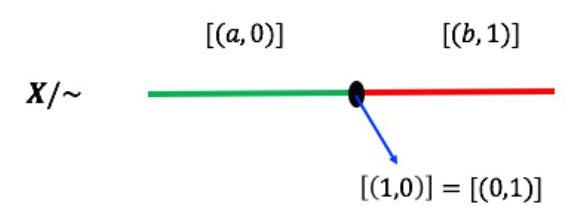
\includegraphics[width=0.4\textwidth]{images/Ch4_two_lines.jpg}
\end{center}

4. Let \(X = \left\lbrack  {0,1}\right\rbrack   \times  \left\lbrack  {0,1}\right\rbrack\). Consider the equivalence class with partition
\[
\{ \left( {a,b}\right) {\} }_{0 < a < 1;0 < b < 1} \cup  \{ \left( {x,0}\right),\left( {x,1}\right) {\} }_{0 \leq  x \leq  1} \cup  \{ \left( {0,y}\right),\left( {1,y}\right) {\} }_{0 < y < 1}
\]
The corresponding quotient space is plotted below:
\begin{center}
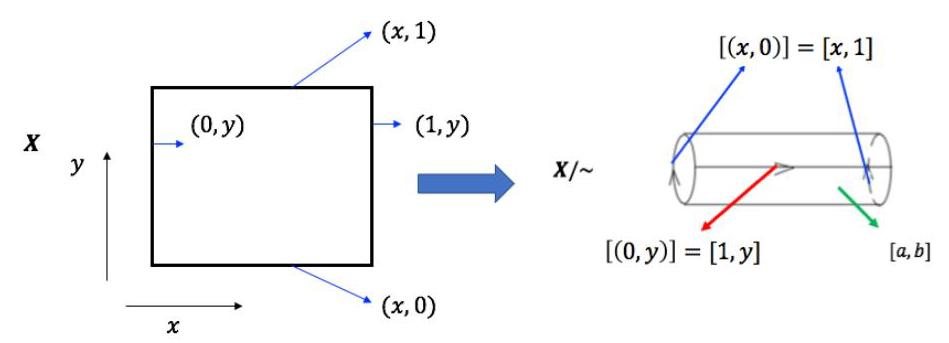
\includegraphics[width=0.8\textwidth]{images/Ch4_cylinder_glue.jpg}
\end{center}
\end{example}

\section{Quotient Topology}

Now given a topologcal space \(X\) and an equivalence relation \(\sim\) on it, our goal is to construct a topology on the space \(X/ \sim\).

\begin{proposition}[Quotient Topology] \label{prop:quotient_topology} Suppose $(X, \mathcal{T})$ is a topological space, and \(\sim\) is an equivalence relation on \(X\). Define the canonical projection map:
\[
p: \;X \rightarrow  X/ \sim  \quad \text{ with } \quad x \mapsto \left\lbrack  x\right\rbrack   
\]
which assigns each point \(x \in  X\) into the equivalence class \(\left\lbrack  x\right\rbrack\). Define a family of subsets \(\widetilde{\mathcal{T}}\) on \(X/ \sim\) by:
\[
\widetilde{U} \subseteq  X/ \sim  \text{ is in }\widetilde{\mathcal{T}}\text{ if }{p}^{-1}\left( \widetilde{U}\right) \text{ is in }\mathcal{T}
\]
Then \(\widetilde{\mathcal{T}}\) is a topology for \(X/ \sim\).  

We say $(X/\sim\, \widetilde{\mathcal{T}})$ the {\bf quotient topology} of the quotient space, and \(X/ \sim\).
\end{proposition}

\begin{proof} 1. \({p}^{-1}\left( {X/ \sim  }\right)  = X \in  \mathcal{T}\) and \({p}^{-1}\left( \varnothing \right)  = \varnothing  \in  \mathcal{T}\), which implies \(X/ \sim   \in  \widetilde{\mathcal{T}}\) and \(\varnothing  \in  \widetilde{\mathcal{T}}\).

2. Suppose that \(\widetilde{U},\widetilde{V} \in  \widetilde{\mathcal{T}}\), then we imply
\[
{p}^{-1}\left( \widetilde{U}\right),{p}^{-1}\left( \widetilde{V}\right)  \in  \mathcal{T} \Rightarrow  {p}^{-1}\left( {\widetilde{U} \cap  \widetilde{V}}\right)  \in  \mathcal{T},
\]
i.e., \(\widetilde{U} \cap  \widetilde{V} \in  \widetilde{\mathcal{T}}\).

3. Following the similar argument in (2), and the relation
\[
{p}^{-1}\left( {\bigcup {\widetilde{U}}_{i}}\right)  = \bigcup {p}^{-1}\left( {\widetilde{U}}_{i}\right),
\]
we conclude that \(\widetilde{T}\) is closed under countably union, and the proof is complete.
\end{proof}

\begin{remark}
1. \autoref{prop:quotient_topology} claims that \(\widetilde{U}\) is open in \(X/ \sim\) iff \({p}^{-1}\left( \widetilde{U}\right)\) is open in \(X\). The general question is that, does \(p\left( U\right)\) is open in \(X/ \sim\), given that \(U\) is open in \(X\) ? This may not necessarily hold. (See example (6.4)) In general \({p}^{-1}\left( {p\left( U\right) }\right)\) is strictly larger than \(U\), and may not be necessarily open in \(X\), even when \(U\) is open.

2. By definition, we can show that \(p\) is continuous.
\end{remark}

To fill the gap on the question shown in the remark, we consider the notion of the open mapping:
\begin{definition}\label{def:open_mapping} [Open Mapping] A function \(f: X \rightarrow  Y\) between two topological spaces is an open mapping if for each open \(U\) in \(X,f\left( U\right)\) is open in \(Y\).
\end{definition}


\begin{example} The mapping \(p: \left\lbrack  {0,1}\right\rbrack   \times  \left\lbrack  {0,1}\right\rbrack   \rightarrow  \left( {\left\lbrack  {0,1}\right\rbrack   \times  \left\lbrack  {0,1}\right\rbrack  }\right) / \sim\) sending the square to the Mobius band \(M\) is not an open mapping: Consider the open ball \(U = {B}_{1/2}\left( \left( {0,0}\right) \right)\) in \(\left\lbrack  {0,1}\right\rbrack   \times  \left\lbrack  {0,1}\right\rbrack\). Note that \(p\left( U\right)\) is open in \(M\) iff \({p}^{-1}\left( {p\left( U\right) }\right)\) is open in \(\left\lbrack  {0,1}\right\rbrack   \times  \left\lbrack  {0,1}\right\rbrack\). We can calculate \({p}^{-1}\left( {p\left( U\right) }\right)\) explicitly:
\[
{p}^{-1}\left( {p\left( U\right) }\right)  = U \cup  \{ \left( {1,y}\right)  \mid  1/2 \leq  y \leq  1\},
\]
which is not open.
\end{example}


\begin{proposition} A subset \(\widetilde{V}\) is closed in the quotient space \(X/ \sim\) iff \({p}^{1}\left( \widetilde{V}\right)\) is closed in \(X\), where \(p: X \rightarrow  X/ \sim\) denotes the canonical projection mapping.
\end{proposition}
\begin{proof} It follows from the fact that
\[
{p}^{-1}\left( {\left( {X/ \sim  }\right)  \smallsetminus  \widetilde{V}}\right)  = X \smallsetminus  {p}^{-1}\left( \widetilde{V}\right)
\]
\end{proof}
\begin{example} \label{eg:circle_glue} Consider \(X = \left\lbrack  {0,1}\right\rbrack\). We define \({x}_{1} \sim  {x}_{2}\) if:
\[
{x}_{1} = 0,{x}_{2} = 1\text{, or }{x}_{1} = 1,{x}_{2} = 0
\]
In other words, the partition on \(X\) is given by:
\[
X = \{ 0,1\}  \cup  \left( {\mathop{\bigcup }\limits_{{x \in  \left( {0,1}\right) }}\{ x\} }\right)
\]
The quotient space "glues" the endpoints of the interval \(\left\lbrack  {0,1}\right\rbrack\) together, shown in the figure below:
\begin{center}
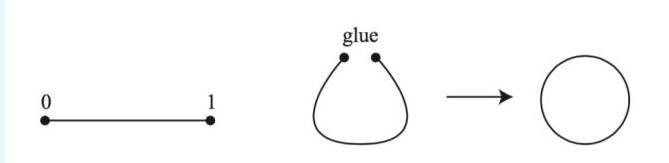
\includegraphics[width=0.6\textwidth]{images/Ch4_circle_glue.jpg}
\end{center}
It is intuitive that the constructed quotient space should be homeomorphic to a circle \({S}^{1}\). We will give a formal proof on this fact.
\end{example}

\begin{proposition} \label{prop:quotient_cont} Let \(X\) and \(Z\) be topological spaces, and \(\sim\) an equivalence relation on \(X\).
Let \(g: X/ \sim   \rightarrow  Z\) be a function, and \(p: X \rightarrow  X/ \sim\) is a projection mapping The mapping \(g\) is continuous if and only if \(g \circ  p: X \rightarrow  Z\) is continuous.
\end{proposition}

\begin{proof} 1. Necessity. Suppose that \(g\) is continuous. It’s clear that \(p\) is continuous, i.e, \(g \circ  p: X \rightarrow  Z\) is continuous.

2. Sufficiency. Suppose that \(g \circ  p: X \rightarrow  Z\) is continuous. Given any open \(U\) in \(Z\), we imply \({\left( g \circ  p\right) }^{-1}\left( U\right)  = {p}^{-1}{g}^{-1}\left( U\right)\) is open in \(X\). By definition of the quotient topology, we imply \({g}^{-1}\left( U\right)\) is open in \(X/ \sim\). Therefore, \(g\) is continuous.
\end{proof}

This useful lemma can be generalized into the case for generalized canonical projection mapping, called quotient mapping.

\begin{definition} \label{def:quotient_map}  A map \(p: X \rightarrow  Y\) between topological spaces is a quotient mapping if
\begin{enumerate}
    \item \(p\) is surjective; and
\item \(p\) is continuous;
\item For any \(U \subseteq  Y\) such that \({p}^{-1}\left( U\right)\) is open in \(X\), we imply \(U\) is open in \(Y\).
\end{enumerate}
\end{definition}

Obviously, the canonical projection map $p: X \to X/\sim$ is a quotient map. The advantage of quotient map is as given below:
\begin{proposition} \label{prop:quotient_cont2} Suppose that \(p: X \rightarrow  Y\) is a quotient map and that \(g: Y \rightarrow  Z\) is any mapping to another space \(Z\). Then \(g\) is continuous iff \(g \circ  p\) is continuous.
\end{proposition}
\begin{proof}
The proof follows similarly as in \autoref{prop:quotient_cont}.
\end{proof} 

Now we give a formal proof of the conclusion in \autoref{eg:circle_glue}:
\begin{proof} Define the mapping
\[
f: \;\left\lbrack  {0,1}\right\rbrack   \rightarrow  {S}^{1}
\quad 
\text{ with } \quad t \mapsto  \left( {\cos {2\pi t},\sin {2\pi t}}\right) \text{. }
\]
Since \(f\left( 0\right)  = f\left( 1\right)\), the function \(f\) induces a well-defined function
\[
g: \;\left\lbrack  {0,1}\right\rbrack  / \sim   \rightarrow  {S}^{1}
\quad
\text{ with }\quad \left\lbrack  t\right\rbrack   \mapsto  f\left( t\right)
\]
such that \(f = g \circ  p\), where \(p\) denotes the canonical projection mapping. Note that \(f\) is continuous. By \autoref{prop:quotient_cont2}, we imply \(g\) is continuous. Furthermore,
\begin{enumerate}
    \item Since \(\left\lbrack  {0,1}\right\rbrack\) is compact and \(p\) is continuous, we imply \(p\left( \left\lbrack  {0,1}\right\rbrack  \right)  = \left\lbrack  {0,1}\right\rbrack  / \sim\) is compact
\item \({S}^{1}\) is Hausdorff
\item \(g\) is a bijection
\end{enumerate}
By applying \autoref{thm:compact_hausdorff_homeo}, we conclude that \(g\) is a homeomorphism, i.e., \(\left\lbrack  {0,1}\right\rbrack  / \sim\) and \({S}^{1}\) are homeomorphic.
\end{proof}

The argument in the proof can be generalized into the proposition below:

\begin{proposition} \label{prop:quotient_homeo} Let \(f: X \rightarrow  Y\) be a surjective continuous mapping between topologcial spaces, and \(\sim\) be an equivalence relation on \(X\) defined by the partition \(\left\{  {{f}^{-1}\left( y\right)  \mid  y \in  Y}\right\}\) (i.e., \(x \sim  {x}^{\prime }\) iff \(f\left( x\right)  = f\left( {x}^{\prime }\right)\)). If \(X\) is compact and \(Y\) is Hausdorff, then \(X/ \sim\) and \(Y\) are homeomorphic.
\end{proposition}

The above proposition allows us to apply the following argument, which we shall use several times: To show 
\[X/ \sim\ \cong Y\] 
are homeomorphic, construct a surjective continuous mapping \(f: X \rightarrow  Y\) such that 
\begin{center}
\(f\left( {x}_{1}\right)  = f\left( {x}_{2}\right)\) whenever \({x}_{1} \sim  {x}_{2}\). 
\end{center}
Therefore, \(f\) will induce a well-defined function \(g: X/ \sim   \rightarrow  Y\) such that \(f = g \circ  p\). Then checking the conditions in \autoref{thm:compact_hausdorff_homeo} leads to the desired results.

\begin{example}
Consider \(X = \left\lbrack  {0,1}\right\rbrack   \times  \left\lbrack  {0,1}\right\rbrack\) and define \(\left( {{s}_{1},{t}_{1}}\right)  \sim  \left( {{s}_{2},{t}_{2}}\right)\) if one of the following holds:
\begin{itemize}
\item \({s}_{1} = {s}_{2}\) and \({t}_{1} = {t}_{2}\) ;
\item \(\left\{  {{s}_{1},{s}_{2}}\right\}   = \{ 0,1\},{t}_{1} = {t}_{2}\) ;
\item \(\left\{  {{t}_{1},{t}_{2}}\right\}   = \{ 0,1\}\) and \({s}_{1} = {s}_{2}\) ;
\item \(\left\{  {{s}_{1},{s}_{2}}\right\}   = \{ 0,1\},\left\{  {{t}_{1},{t}_{2}}\right\}   = \{ 0,1\}\)
\end{itemize}
We now show the corresponding quotient space \(\left( {\left\lbrack  {0,1}\right\rbrack   \times  \left\lbrack  {0,1}\right\rbrack  }\right) / \sim\) is hoemomorhpic to the torus \({\mathbb{T}}^{2}\): Define the mapping 
\[f: \left\lbrack  {0,1}\right\rbrack   \times  \left\lbrack  {0,1}\right\rbrack   \rightarrow  {\mathbb{T}}^{2} \quad \quad \left( {{t}_{1},{t}_{2}}\right)  \mapsto  \left( {{e}^{{2\pi i}{t}_{1}},{e}^{{2\pi i}{t}_{2}}}\right).\]
Then
\begin{itemize}
    \item \(f\) is surjective, which also implies \({\mathbb{T}}^{2} = f\left( {\left\lbrack  {0,1}\right\rbrack   \times  \left\lbrack  {0,1}\right\rbrack  }\right)\) is compact.

 \item \({\mathbb{T}}^{2}\) is Hausdorff.

\item It’s clear that \(\left( {{s}_{1},{t}_{1}}\right)  \sim  \left( {{s}_{2},{t}_{2}}\right)\) implies \(f\left( {{s}_{1},{t}_{1}}\right)  = f\left( {{s}_{2},{t}_{2}}\right)\). Conversely, suppose
\[
{e}^{{2\pi i}{s}_{1}} = {e}^{{2\pi i}{s}_{2}},\;{e}^{{2\pi i}{t}_{1}} = {e}^{{2\pi i}{t}_{2}}
\]
By the familiar property of \({e}^{ix}\), we imply either \({t}_{1} = {t}_{2}\) or \(\left\{  {{t}_{1},{t}_{2}}\right\}   = \{ 0,1\}\); and either \({s}_{1} = {s}_{2}\) or \(\left\{  {{s}_{1},{s}_{2}}\right\}   = \{ 0,1\}\)
\end{itemize}
By applying \autoref{prop:quotient_homeo}, we conclude that \(\left( {\left\lbrack  {0,1}\right\rbrack   \times  \left\lbrack  {0,1}\right\rbrack  }\right) / \sim\) is homeomorphic to \({\mathbb{T}}^{2}\).
\end{example}

\begin{example}
Consider the closed disk \({\mathbb{D}}^{2} = \left\{  {\left( {x,y}\right)  \in  {\mathbb{R}}^{2} \mid  {x}^{2} + {y}^{2} \leq  1}\right\}\), and define \(\left( {{x}_{1},{y}_{1}}\right)  \sim  \left( {{x}_{2},{y}_{2}}\right)\) by:
\begin{itemize}
\item \({x}_{1} = {x}_{2}\) and \({y}_{1} = {y}_{2}\) ;
\item \(\left( {{x}_{1},{y}_{1}}\right)\) and \(\left( {{x}_{2},{y}_{2}}\right)\) are in the boundary circle \({\mathbb{S}}^{1}\)
\end{itemize}
Then the corresponding quotient space \({\mathbb{D}}^{2}/ \sim\) is hoemomorhpic to the 2-dimension sphere \({\mathbb{S}}^{2} = \left\{  {\left( {x,y,z}\right)  \mid  {x}^{2} + {y}^{2} + {z}^{2} = 1}\right\}\): Define the mapping
\[f: \;{\mathbb{D}}^{2} \rightarrow  {\mathbb{S}}^{2} \]
by 
\begin{align*} 
\left( {0,0}\right)  &\mapsto  \left( {0,0,1}\right)\\
\left( {x,y}\right)  &\mapsto  \left( {\frac{x}{\sqrt{{x}^{2} + {y}^{2}}}\sin \left( {\pi \sqrt{{x}^{2} + {y}^{2}}}\right),\frac{y}{\sqrt{{x}^{2} + {y}^{2}}}\sin \left( {\pi \sqrt{{x}^{2} + {y}^{2}}}\right),\cos \left( {\pi \sqrt{{x}^{2} + {y}^{2}}}\right) }\right)
\end{align*}
It’s easy to check the conditions in \autoref{prop:quotient_homeo}, and we conclude that \({\mathbb{D}}^{2}/ \sim\)
is hoemomorhpic to \({\mathbb{S}}^{2}\).
\end{example}

In \autoref{prop:quotient_homeo}, we show the homeomorphism between \(X/ \sim\) and \(Y\) given the compactness of \(X\) and Hausdorffness of \(Y\). Now we show the generalize the proposition by replacing these conditions with the quotient mapping \(q\):
\begin{proposition} Suppose \(q: X \rightarrow  Y\) is a quotient map, and that \(\sim\) is an equivalence relation on \(X\) given by the partition \(\left\{  {{q}^{-1}\left( y\right)  \mid  y \in  Y}\right\}\). Then \(X/ \sim\) and \(Y\) are homeomorphic.
\end{proposition}
\begin{proof} Construct the mapping
\[
h: \;X/ \sim   \rightarrow  Y  \quad 
\text{ with } \quad h\left( \left\lbrack  x\right\rbrack  \right)  = q\left( x\right)
\]
Note that the mapping \(h\) is well-defined and bijective. And the quotient mapping \(q \mathrel{\text{:= }} h \circ  p\) is continuous by definition. By applying \autoref{prop:quotient_cont}, \(h\) is continuous, and we are only left to show that $h^{-1}$ is continuous, i.e. 
for any open \(\widetilde{U} \subseteq  X/ \sim\), \(h\left( \widetilde{U}\right)\) is open in \(Y\).

To see so, note that
\[
{q}^{-1}\left( {h\left( \widetilde{U}\right) }\right)  = {p}^{-1}{h}^{-1}\left( {h\left( \widetilde{U}\right) }\right)  = {p}^{-1}\left( \widetilde{U}\right),
\]
which is open by the definition of quotient topology. Therefore, \(h\left( \widetilde{U}\right)\) is open by (2) in \autoref{def:quotient_map}.
\end{proof}

\begin{example} \(\mathbb{R}/\mathbb{Z}\) is homeomorphic to the unit circle \({S}^{1}\): Indeed, consider the mapping
\[
q: \mathbb{R} \rightarrow  {S}^{1}
\quad \quad
x \mapsto  {e}^{2\pi ix}
\]
It is clear that

1. \(q\) is a continuous open mapping (why?)

2. \(q\) is surjective

Therefore, \(\mathbb{R}/ \sim   \cong  {S}^{1}\), provided that \(x \sim  y\) iff \(q\left( x\right)  = q\left( y\right)\), i.e., \(x - y \in  \mathbb{Z}\). Therefore,
\[
\mathbb{R}/\mathbb{Z} \cong  {S}^{1}
\]
\end{example}

\section{Simplicial Complex}
The idea of simplicial complex is to build some new spaces from some "fundamental" objects. The combinatorists often study topology by the combinatorics of these fundamental objects. First we define what are the "fundamental" objects:

\begin{definition}[ \(n\) -simplex] \label{def:n_simplex} The standard \(n\) -simplex is the set
\[
{\Delta }^{n} = \left\{  {\left( {{x}_{1},\ldots,{x}_{n + 1}}\right)  \in  {\mathbb{R}}^{n + 1} \mid  {x}_{i} \geq  0,\forall i\text{ and }\mathop{\Sigma }\limits_{{i = 1}}^{{n + 1}}{x}_{i} = 1}\right\}
\]
The $0$, $1$, $2$ and $3$ simplices can be visualized as follows:
\begin{center}
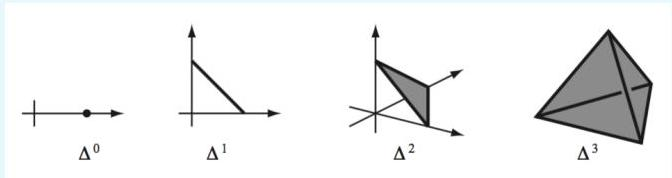
\includegraphics[width=0.7\textwidth]{images/Ch4_simplices.jpg}
\end{center}

1. The non-negative integer \(n\) is the \emph{dimension} of this simplex;

2. Its \emph{vertices}, denoted as \(V\left( {\Delta }^{n}\right)\), are those points \(\left( {{x}_{1},\ldots,{x}_{n + 1}}\right)\) in \({\Delta }^{n}\) such that \({x}_{i} = 1\) for some \(i\).

3. For each given non-empty \(\mathcal{A} \subseteq  \{ 1,\ldots,n + 1\}\), its \emph{facet} is defined as
\[
\left\{  {\left( {{x}_{1},\ldots,{x}_{n + 1}}\right)  \in  {\Delta }^{n} \mid  {x}_{i} = 0,\forall i \notin  \mathcal{A}}\right\}
\]
In particular, \({\Delta }^{n}\) is a face of itself

4. The \emph{inside} of \({\Delta }^{n}\) is
\[
\operatorname{inside}\left( {\Delta }^{n}\right)  \mathrel{\text{:= }} \left\{  {\left( {{x}_{1},\ldots,{x}_{n + 1}}\right)  \in  {\Delta }^{n} \mid  {x}_{i} > 0,\forall i}\right\}
\]
In particular, the inside of \({\Delta }^{0}\) is \({\Delta }^{0}\).
\end{definition}

\begin{definition}[Face Inclusion] A \emph{face inclusion} of \({\Delta }^{m}\) into \({\Delta }^{n}\left( {m < n}\right)\) is a function \({\Delta }^{m} \rightarrow  {\Delta }^{n}\) which comes from the restriction of an injective linear map \(f: {\mathbb{R}}^{m + 1} \rightarrow  {\mathbb{R}}^{n + 1}\) that maps vertices in \({\Delta }^{m}\) into vertices in \({\Delta }^{n}\).
\end{definition}

For example, the linear transformation \(f: {\mathbb{R}}^{2} \rightarrow  {\mathbb{R}}^{3}\) defined below is a face inclusion:
\[
f\left( {1,0}\right)  = \left( {0,1,0}\right),\;f\left( {0,1}\right)  = \left( {0,0,1}\right).
\]

\begin{remark} Any injection mapping from \(\{ 1,\ldots,m + 1\}  \rightarrow  \{ 1,\ldots,n + 1\}\) gives a face inclusion \({\Delta }^{m} \rightarrow  {\Delta }^{n}\), and vice versa.
\end{remark}

Now we build new spaces by gluing simplices together. This new space is called the simplicial complex. If a simplex is a part of the complex, so are all its faces.
\begin{definition}[Abstract Simplicial Complex] \label{def:simplicial_complex} An (abstract) simplicial complex is a pair \(K = \left( {V,\Sigma }\right)\), where \(V\) is a set of vertices and \(\Sigma\) is a collection of non-empty finite subsets of \(V\) (simplices) such that

1. For any \(v \in  V\), the 1-element set \(\{ v\}\) is in \(\Sigma\)

2. If \(\sigma\) is an element of \(\Sigma\), then so is any non-empty subset of \(\sigma\).
\end{definition}

For example, if \(V = \{ 1,2,3,4\}\), then one can take:
\begin{equation} \label{eq:sigma}
\Sigma  = \{ \{ 1\},\{ 2\},\{ 3\},\{ 4\},\{ 1,3,4\},\{ 2,4\},\{ 1,3\},\{ 3,4\},\{ 1,4\}. \}    
\end{equation}

We can associate to an abstract simplicial complex \(K\) a topological space \(\left| K\right|\), which is called its geometric realization:

\begin{definition}[Topological Realization] \label{def:topological_realization} The topological realization of \(K = \left( {V,\Sigma }\right)\) is a topological space \(\left| K\right|\) (or denoted as \(\left| \left( {V,\Sigma }\right) \right|\) ), where

1. For each \(\sigma  \in  \Sigma\) with \(\left| \sigma \right|  = n + 1\), take a copy of \(n\) -simplex and denote it as \({\Delta }_{\sigma }\)

2. Whenever \(\sigma  \subset  \tau  \in  \Sigma\), identify \({\Delta }_{\sigma }\) with a face of \({\Delta }_{\tau }\) through face inclusion.

Or equivalently, \(\left| K\right|\) is a quotient space of the disjoint union
\[
\mathop{\coprod }\limits_{{\sigma  \in  \Sigma }}\sigma
\]
by the equivalence relation which identifies a point \(y \in  \sigma\) with its image under the face inclusion \(\sigma  \rightarrow  \tau\), for any \(\sigma  \subset  \tau\).
\end{definition}

\begin{example} Take $(V,\Sigma)$ as in \autoref{eq:sigma}, so that
\begin{center}
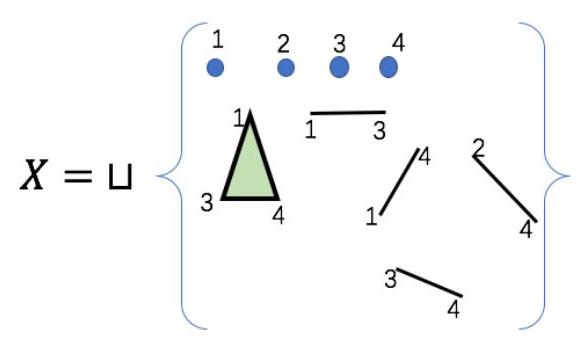
\includegraphics[width=0.6\textwidth]{images/Ch4_glue1.jpg}
\end{center}
Then its topological realization is:
\begin{center}
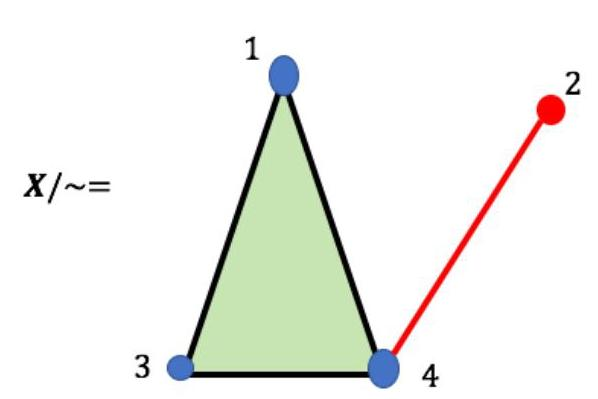
\includegraphics[width=0.4\textwidth]{images/Ch4_glue2.jpg}
\end{center}
\end{example} 

\begin{example} Take \(V = \{ 1,2,3,4\}\) and \(\Sigma  = \{\) all subsets of \(V\) except \(V\}\). 
Then its topological realization is \(\left| \left( {V,\Sigma }\right) \right|  = {\Delta }^{3}\) as shown in the figure below:
\begin{center}
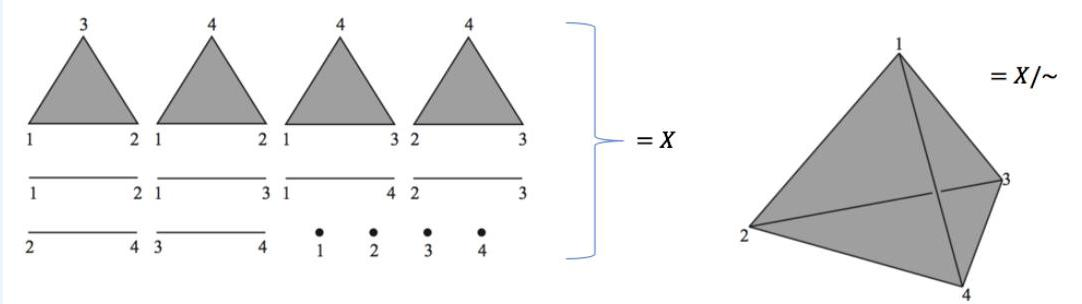
\includegraphics[width=0.9\textwidth]{images/Ch4_glue_3_simplex.jpg}
\end{center}
\end{example}

\begin{definition}[Triangulation] A \emph{triangulation} of a topological space \(X\) is a simplicial complex \(K = \left( {V,\Sigma }\right)\) together with a choice of homeomorphism \(\left| K\right|  \rightarrow  X\).
\end{definition}


\begin{example} \label{eg:tours_triangulation}
Consider the simplical complex \(K = \left( {V,\Sigma }\right)\) with
\[
V = \{ 1,2,3,4,\ldots,9\},\;\Sigma  = \left\{  \begin{array}{r} 9\text{ subsets with }1\text{ element } \\  {27}\text{ subsets with }2\text{ elements } \\  {18}\text{ subsets with }3\text{ elements } \end{array}\right.
\]
as given below. We start to build the topological realization of \(K\) with $9$ 0-simplicies, $27$ 1-simplicies, and $18$ 2-simplicies. The identification of them is as follows:
\begin{center}
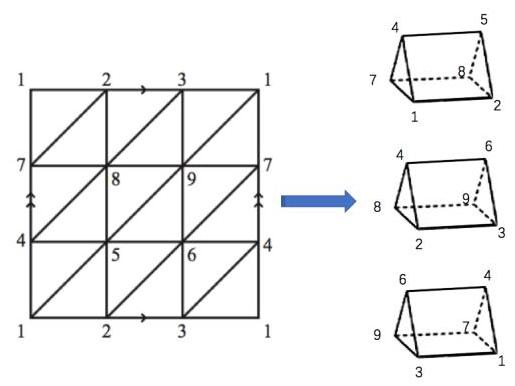
\includegraphics[width=0.6\textwidth]{images/Ch4_torus_triangle.jpg}
\end{center}
Step 1: Identify 3 columns separately, i.e., identify \(\{ 1,7,4,1,2,8,5,2\}\), \(\{ 2,8,5,2,3,9,6,3\}\), and \(\{ 3,9,6,3,1,7,4,1\}\).

\begin{center}
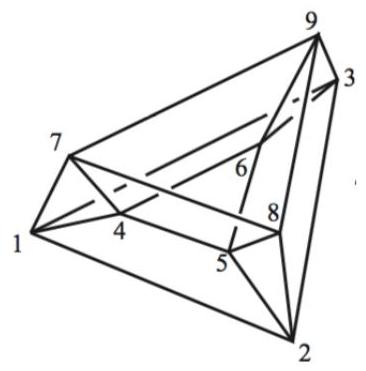
\includegraphics[width=0.3\textwidth]{images/Ch4_torus_triangle2.jpg}
\end{center}
Step 2: "glue" these three prisms in the figure above together. Then it will give us a `torus'. We will see in a moment that this $K = (V,\Sigma)$ is indeed a triangulation of $\mathbb{T}$.
\end{example}

\begin{example}
The simplicial complex below is a topological realization of \({S}^{2}\):
\begin{center}
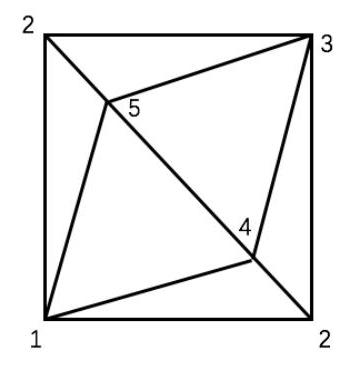
\includegraphics[width=0.35\textwidth]{images/Ch4_S1_triangle.jpg}
\end{center}
Indeed, $S^2$ is homeomorphic to the quotient space of $[0,1] \times [0,1]$ with the following identification:
\begin{center}
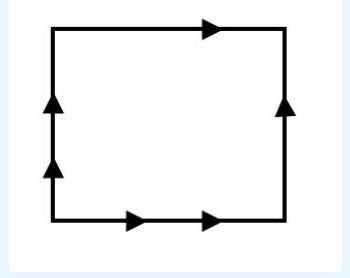
\includegraphics[width=0.35\textwidth]{images/Ch4_S1_quotient.jpg}
\end{center}
\end{example}

\begin{example}
One may ask whether one we build a triangulation of the tours using fewer simplices as in \autoref{eg:tours_triangulation}? The answer is no. 

For instance, one may think the number of triangles can be reduced as in the figure below: 
\begin{center}
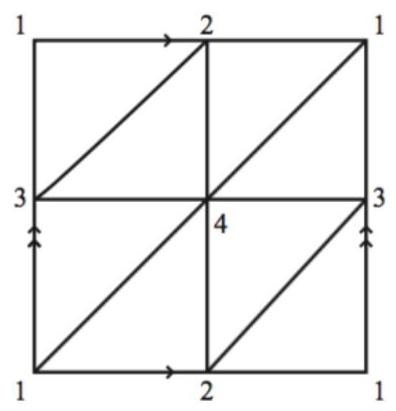
\includegraphics[width=0.3\textwidth]{images/Ch4_turous_nonex.jpg}
\end{center}
However, if one pays attention to the bottom edge of the square, there are two 1-simplicies labeled \(\{ 1,2\}\), which means we have to 'glue the two bottom edges together, which cannot happen in the construction of torus.

As another example, the following diagram {\bf DOES NOT} give a triangulation of $S^2$:
\begin{center}
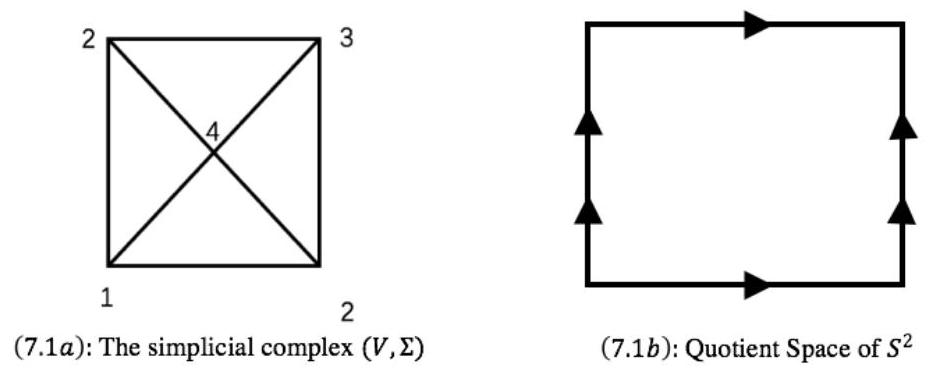
\includegraphics[width=0.6\textwidth]{images/Ch4_S2_nonex.jpg}
\end{center}
Note that the 2-simplex \({\Delta }_{\{ 2,3,4\} }\) appears twice in the left hand side of the figure. This means that we need to stick the top triangle and the right triangle together, which contradicts to the structure of the quotient space \({S}^{2}\) shown on the right hand side.
\end{example}

Simplicial complex gives us a combinatorial way to study \(X\), i.e. it suffices to study \(\left( {V,\Sigma }\right)\) such that \(\left| \left( {V,\Sigma }\right) \right|  \cong  X\). 
For example, if we want to distinguish \(\mathbb{T} = {S}^{1} \times  {S}^{1}\) and \({S}^{2}\), we just need  distinguish between their topological realizations. One way to do so is the following:

\begin{theorem}[Euler Characteristic] \label{thm:euler_char}
For any simplicial complex $(V,\Sigma)$, the Euler characteristic is defined by
\[\mathcal{X}(V,\Sigma) :=
\mathop{\sum }\limits_{{i = 1}}^{\infty }{\left( -1\right) }^{i}\text{ (number of subsets in }{\Sigma }\text{ with }\left( {i + 1}\right) \text{ -element) }
\]
Suppose that \(\left| \left( {{V}_{1},{\Sigma }_{1}}\right) \right|  \cong  \left| \left( {{V}_{2},{\Sigma }_{2}}\right) \right|\), then
\[\mathcal{X}\left( {{V}_{1},{\Sigma }_{1}}\right) = \mathcal{X}\left( {{V}_{2},{\Sigma }_{2}}\right).
\]
In particular, for two triangulations of the same topological space $X$, it has the same Euler characteristic. So we can define
$$\mathcal{X}(X) := \mathcal{X}(V,\Sigma)$$
for \emph{any} triangulation $|(V,\Sigma)| \cong X$ of $X$.
\end{theorem}

From previous examples, we can see that \(\mathcal{X}\left( {S}^{2}\right)  = 5 - 9 + 6 = 2\) and \(\mathcal{X}\left( \mathbb{T}\right)  = 9 - {27} + {18} = 0\), which implies
\[
{S}^{2} \ncong \mathbb{T}.
\]

\section{Properties of Simplicial Complex}
\begin{definition}[Simplicial Subcomplex] A subcomplex of a simplicial complex \(K = \left( {V,\Sigma }\right)\) is a simplicial complex \({K}^{\prime } = \left( {{V}^{\prime },{\Sigma }^{\prime }}\right)\) such that
\[
{V}^{\prime } \subseteq  V,\;{\Sigma }^{\prime } \subseteq  \Sigma
\]
\end{definition}

\begin{proposition} Suppose \({K}^{\prime }\) is subcomplex of \(K\), then \(\left| {K}^{\prime }\right|\) is closed in \(\left| K\right|\).
\end{proposition}
\begin{proof} Suppose that \(D\) is the disjoint union of all the simplicial complex forming \(\left| K\right|\) (note that the number of component in \(D\) is \(\left| \Sigma \right|\) )
Consider the canonical projection mapping 
\[p: D \rightarrow  \left| K\right|.\] Observe that \({p}^{-1}\left( \left| {K}^{\prime }\right| \right)\) precisely equals to \(\mathop{\coprod }\limits_{{{\sigma }^{\prime } \in  {\Sigma }^{\prime }}}{\sigma }^{\prime }\), which is closed in \(D\). By definition of quotient topology, \(\left| {K}^{\prime }\right|\) is also closed.
\end{proof}

\begin{definition} Let \(K = \left( {V,\Sigma }\right)\) be a simplicial complex and \({V}^{\prime } \subseteq  V\). Then the subcomplex spanned by \({V}^{\prime }\) is \(\left( {{V}^{\prime },{\Sigma }^{\prime }}\right)\) such that
\begin{itemize}
\item \({V}^{\prime }\) denotes the vertex set.
\item the simplices \({\Sigma }^{\prime }\) is given by
\[
\left\{  {\sigma  \in  \Sigma  \mid  \sigma  \subseteq  {V}^{\prime }}\right\}
\]
\end{itemize}
\end{definition}

\begin{definition} [Link and Star] \label{def:link_star} Let \(\left( {V,\Sigma }\right)  = K\) be a simplicial complex.
\begin{itemize}
\item The \emph{link} of \(v \in  V\), denoted as \(\operatorname{lk}\left( v\right)\) is the sub-complex with vertex set:
\[
\{ w \in  V \smallsetminus  \{ v\}  \mid  \{ v,w\}  \in  \Sigma \}
\]
and simplicies:
\[
\{ \sigma  \in  \Sigma  \mid  \mathbf{v} \notin  \sigma \text{ and }\sigma  \cup  \{ \mathbf{v}\}  \in  \Sigma \}
\]
\item The \emph{star} of \(v\) (denoted as \(\operatorname{st}\left( v\right)\)) is
\[
\bigcup_{\sigma  \in  \Sigma,\ v \in  \sigma} \operatorname{inside}\left( \sigma \right)
\]
(c.f. \autoref{def:n_simplex} for the definition of inside of an $n$-simplex)
\end{itemize}
\end{definition}

\begin{proposition} \(\mathrm{{st}}\left( v\right)\) is open and \(v \in  \mathrm{{st}}\left( v\right)\).
\end{proposition}
\begin{proof} Omitted - In fact, \(\left| K\right|  \smallsetminus  \operatorname{st}\left( v\right)\) is the simplicial subcomplex spanned by \(V\).
\end{proof}

\begin{proposition} Suppose that \(K = \left( {V,\Sigma }\right)\), where \(V\) is finite. Then \(\left| K\right|\) is compact.
\end{proposition}
\begin{proof} The mapping \(p: D \rightarrow  \left| K\right|\) is a canonical projection mapping, which is continuous; and \(D\) (the finite disjoint union of \({\Delta }_{\sigma }\) ’s) is compact. Therefore, \(p\left( D\right)  = \left| K\right|\) is compact.
\end{proof}

\begin{proposition} For any simplicial complex \(K = \left( {V,\Sigma }\right)\), where \(V\) is finite, there is a continuous injection
\[
f: \left| K\right|  \rightarrow  {\mathbb{R}}^{n}\text{ for some }n
\]
\end{proposition}

\begin{proof} Let \(K^{\Pi} = \left( {V,\Sigma^{\Pi}}\right)\), where \(\Sigma^{\Pi} =\) power set of \(V\). Then
\[
\left| K^{\Pi}\right|  = {\Delta }^{\left| V\right|  - 1} \subseteq  {\mathbb{R}}^{\left| V\right| }
\]
Consider the inclusion
\[
i: \left| K\right|  \rightarrow  \left| K^{\Pi}\right|
\]
which comes from the following:
\begin{enumerate}
    \item Consider the \(D \mathrel{\text{:= }} \mathop{\coprod }\limits_{{\sigma  \in  \Sigma }}{\Delta }_{\sigma }\) and \({D}^{\prime } = \mathop{\coprod }\limits_{{\Sigma^{\Pi} \in  \Sigma^{\Pi}}}{\Delta }_{\Sigma^{\Pi}}\) in \(\left( {V,\Sigma }\right)\) and \(\left( {V,\Sigma^{\Pi}}\right)\)

\item Construct the mapping \(\widetilde{i}: D \hookrightarrow  {D}^{\prime }\overset{{p}^{\prime }}{ \rightarrow  }\left| K\right|\).

\item The mapping \(\widetilde{i}\) descends to \(i: D/ \sim   \rightarrow  \left| K^{\Pi}\right|\) (try to write down the detailed mapping), which is continuous and injective.
\end{enumerate}
Therefore, \(\left| K\right|  \hookrightarrow  \left| K^{\Pi}\right|  (\hookrightarrow  {\mathbb{R}}^{n})\), and the proof is complete.
\end{proof}

\begin{remark} 
More generally, if \(K = \left( V,\Sigma \right)\) is a simplicial subcomplex of \(\widetilde{K} = \left( {\widetilde{V},\widetilde{\Sigma}}\right)\), we can construct a continuous injection from \(\left| K\right|\) to \(\left| \widetilde{K}\right|\).

Let \({D}_{\Sigma } \mathrel{\text{:= }} \mathop{\coprod }\limits_{{\sigma  \in  \Sigma }}\sigma\) and \({D}_{\widetilde{\Sigma}} \mathrel{\text{:= }} \mathop{\coprod }\limits_{{\widetilde{\sigma} \in  \widetilde{\Sigma}}}\widetilde{\sigma}\), then \(\left| K\right|  = {D}_{\Sigma }/{ \sim  }_{\Sigma }\) and \(\left| \widetilde{K}\right|  = {D}_{\widetilde{\Sigma}}/{ \sim  }_{\widetilde{\Sigma}}\). It follows that
\[f:  {D}_{\Sigma } \rightarrow {D}_{\widetilde{\Sigma}} 
\overset{p}{ \rightarrow  }{D}_{\Sigma }/{ \sim  }_{\Sigma },\] 
where $p$ denotes the canonical projection mapping. Then \(f\) descends to a continuous mapping
\[
\widetilde{f}: {D}_{\Sigma }/{ \sim  }_{\Sigma } \rightarrow {D}_{\widetilde{\Sigma}}/{ \sim  }_{\widetilde{\Sigma}}
\]
Note that \(\widetilde{f}\) is injective since for all $x,y \in  {D}_{\Sigma }$,
\[
x{ \sim  }_{\widetilde{\Sigma}}y \quad \Leftrightarrow  \quad i\left( x\right) { \sim  }_{\widetilde{\Sigma}}\ i\left( y\right),
\]
where \(i: D_{\Sigma} \hookrightarrow D_{\widetilde{\Sigma}}\) denotes the inclusion mapping.
\end{remark}


\begin{proposition} If \(K = \left( {V,\Sigma }\right)\) with finite \(V\), then \(\left| K\right|\) is Hausdorff.
\end{proposition}

\begin{proof} Let \(g: \left| K\right| \hookrightarrow  {\mathbb{R}}^{n}\). Consider the bijective \(g: \left| K\right|  \rightarrow  g\left( \left| K\right| \right)\), which is continuous.
Since \(\left| K\right|\) is compact, and \(g\left( \left| K\right| \right)  \subseteq  {\mathbb{R}}^{n}\) is Hausdorff, we imply that \(\left| K\right|\) and \(g\left( \left| K\right| \right)\) are homeomorphic, i.e., \(\left| K\right|\) is Hausdorff.
\end{proof}

\begin{definition}[Edge Path] \label{def:edge_path} An edge path of \(K = \left( {V,\Sigma }\right)\) is a sequence of vertices \(\left( {{v}_{1},\ldots,{v}_{n}}\right),{v}_{i} \in  V\) such that \(\left\{  {{v}_{i},{v}_{i + 1}}\right\}   \in  \Sigma,\forall i\).
\end{definition}

\begin{proposition} Let \(K = \left( {V,\Sigma }\right)\) be a simplicial complex. The following are equivalent:

1. \(\left| K\right|\) is connected.

2. \(\left| K\right|\) is path-connected.

3. Any 2 vertices in \(\left( {V,\Sigma }\right)\) can be joined by an edge path, i.e., for \(\forall u,v \in  V\), there exists \({v}_{1},\ldots,{v}_{k} \in  V\) such that \(\left( {u,{v}_{1},\ldots,{v}_{k},v}\right)\) is an edge path.
\end{proposition}

Sketch of Proof (to be revised). 1. (3) implies (2): For every \(x,y \in  \left| K\right|\),

\[
\left\{  \begin{array}{l} x \in  {\Delta }_{{\sigma }_{1}}\text{ for some }{\sigma }_{1} \in  \Sigma. \\  y \in  {\Delta }_{{\sigma }_{2}}\text{ for some }{\sigma }_{2} \in  \Sigma. \end{array}\right.
\]

Take a path joining \(x\) to a vertex \({v}_{1} \in  {\sigma }_{1}\) and a path joining \(y\) to a vertex \({v}_{2} \in  {\sigma }_{2}\). By (3), we have a path joining \({v}_{1}\) and \({v}_{2}\).

2. (1) implies (3): Suppose on the contrary that there is a vertex \(v\) not satisfying (3). Take \({V}^{\prime }\) as the set of vertexs that can be joined with \(v\) ; and \({V}^{\prime \prime }\) as the set of vertexs that cannot be joinied with \(v\).

Then \({V}^{\prime },{V}^{\prime \prime } \neq  \varnothing\). Consider \({K}^{\prime },{K}^{\prime \prime }\) be simplicial subcomplexes of \(K\), spanned by \({V}^{\prime }\) and \({V}^{\prime \prime }\). Then \(\left| {K}^{\prime }\right|,\left| {K}^{\prime \prime }\right|\) are disjoint, closed in \(\left| K\right|\).

\(\left| K\right|  = \left| {K}^{\prime }\right|  \cup  \left| {K}^{\prime \prime }\right|\). If there exists \(x \in  \left| K\right|  \smallsetminus  \left( {\left| {K}^{\prime }\right|  \cup  \left| {K}^{\prime \prime }\right| }\right)\), then for any \(\sigma  \in  \Sigma\) such that \(x \in  {\Delta }_{\sigma }\), we imply \({\Delta }_{\sigma } \nsubseteq  \left| {K}^{\prime }\right|\) or \(\left| {K}^{\prime \prime }\right|\).

Therefore, \(\sigma\) consists of vertices in both \({V}^{\prime }\) and \({V}^{\prime \prime }\). Then there is \({v}^{\prime },{v}^{\prime \prime } \in  \sigma\) joining \({V}^{\prime }\) and \({V}^{\prime \prime }\).

Therefore, there is no such \(x\) and hence \(\left| K\right|  = \left| {K}^{\prime }\right|  \cup  \left| {K}^{\prime \prime }\right|\) is a disjoint union of two closed sets, i.e., not connected.